
%%% Local Variables:
%%% mode: latex
%%% TeX-master: t
%%% End:
\documentclass[serif ,mathserif ,professionalfont,hyperref={pdfpagelabels=false}]{beamer}
%\usepackage{lmodern}
\usepackage{exscale}
\usepackage{amsmath}
\usepackage{graphicx}
%\usepackage{mathptmx} % seems something to do with the font
\usepackage{helvet}
\usepackage{tcolorbox}
\usepackage{textpos}
\usepackage{xargs}
\usepackage{tikz}
\usepackage{amssymb}
\usepackage[]{algorithm2e}
\usepackage{pxfonts}
\usepackage{eulervm}
\usepackage[miktex]{gnuplottex} % for MiKTeX,`pdflatex -shell-escape`
                                % enabled
\usepackage[export]{adjustbox}
\usepackage{cite}
\usepackage{mathtools}
\DeclareMathOperator*{\argmin}{argmin}
\DeclareMathOperator*{\argmax}{argmax}

\renewcommand{\familydefault}{helvetica}
%\renewcommand{\labelitemi}{$\bluesquare$}
\newcommand{\labelitemi}{\textbf{\ding{192}}}
\newcommand{\localtextbulletone}{\textcolor{gray}{\raisebox{.45ex}{\rule{.6ex}{.6ex}}}}
\newcommand\norm[1]{\left\lVert#1\right\rVert}
\renewcommand{\labelitemi}{\localtextbulletone}
%\renewcommand\mathfamilydefault{\mathnormal}
%\renewcommand{\theequation}{\thechapter--\arabic{equation}} % for
                                % equation number style



\DeclareMathOperator{\dom}{dom}
\def\gdw{\mathrel{{>}\mkern-13mu{<}}}

\setbeamertemplate{itemize items}[square]


\usetheme{Frankfurt}
\setbeamercolor{section in head/foot}{fg=white, bg=blue!20!black!90}


%% commands definitions for
\newcommand\mynew{andyandyandy}

%% end of the definition of commands

%%% block definition
\newenvironment<>{redblock}[1]{%
  \setbeamercolor{block title}{fg=white,bg=red!75!black!65}%
  \setbeamercolor{block body}{fg=red!40!black!70,bg=red!60!black!20}%

  \begin{block}#2{#1}}{\end{block}}
\newenvironment<>{blueblock}[1]{%
  \setbeamercolor{block title}{fg=white,bg=blue!75!black!65}%
  \setbeamercolor{block body}{fg=black,bg=blue!60!black!20}%
  \begin{block}#2{#1}}{\end{block}}

\newenvironment<>{greyblock}[1]{%
  \setbeamercolor{block title}{fg=white,bg=black!75}%
  \setbeamercolor{block body}{fg=black,bg=black!40}%
  \begin{block}#2{#1}}{\end{block}}

\newenvironment<>{greenblock}[1]{%
  \setbeamercolor{block title}{fg=white,bg=green!75!black!65}%
  \setbeamercolor{block body}{fg=black,bg=green!60!black!20}%
  \begin{block}#2{#1}}{\end{block}}
%%% Block definition


% for the note style
% \newcommandx{\unsure}[2][1=]{\todo[linecolor=red,backgroundcolor=red!25,bordercolor=red,#1]{#2}}
% \newcommandx{\change}[2][1=]{\todo[linecolor=blue,backgroundcolor=blue!25,bordercolor=blue,#1]{#2}}
% \newcommandx{\info}[2][1=]{\todo[linecolor=OliveGreen,backgroundcolor=OliveGreen!25,bordercolor=OliveGreen,#1]{#2}}
% \newcommandx{\improvement}[2][1=]{\todo[linecolor=Plum,backgroundcolor=Plum!25,bordercolor=Plum,#1]{#2}}
% \newcommandx{\thiswillnotshow}[2][1=]{\todo[disable,#1]{#2}}

%% configuration for the slids style
\makeatletter
\setbeamertemplate{footline}
{
  \leavevmode%
  \hbox{%
    \begin{beamercolorbox}[wd=.333333\paperwidth,ht=2.25ex,dp=1.6ex,center]{author in head/foot}%
      \usebeamerfont{author in
        head/foot}%
      \insertshortauthor\hspace{1em}\beamer@ifempty{Advanced
        Algorithms}{}{Advanced
        Algorithms}
    \end{beamercolorbox}%
    \begin{beamercolorbox}[wd=.333333\paperwidth,ht=2.25ex,dp=1.6ex,center]{title in head/foot}%
      \usebeamerfont{title in head/foot}\insertshorttitle
    \end{beamercolorbox}%
    \begin{beamercolorbox}[wd=.333333\paperwidth,ht=2.25ex,dp=1.6ex,right]{date in head/foot}%
      \usebeamerfont{date in head/foot}\insertshortdate{}\hspace*{2em}
      \insertframenumber{} / \inserttotalframenumber\hspace*{2ex}
    \end{beamercolorbox}}%
  \vskip0pt%
}
\makeatother

\author[\parbox{.2\paperwidth}{}]{Pan An}
\institute{National University of Singapore}
\title{VR Controlling}

%% end of configuration


\date{\today}
\setbeamertemplate{bibliography item}[triangle]
\begin{document}

\begin{frame}
  \titlepage
\end{frame}





\section{Introduction}

%%% Local Variables:
%%% mode: latex
%%% TeX-master: "sinapse"
%%% End:


\begin{frame}
  \frametitle{System Brief}
  \only<1>{
    \begin{block}{Perception}
      \begin{itemize}
      \item Visual
      \item Touching
      \end{itemize}
    \end{block}

    \begin{block}{Controlling}
      \begin{itemize}
      \item Spatial
      \item 
      \end{itemize}
    \end{block}
  }
\end{frame}

\begin{frame}
  \frametitle{Interaction and Feedback}
  \begin{figure}[!ht]
    \centering
    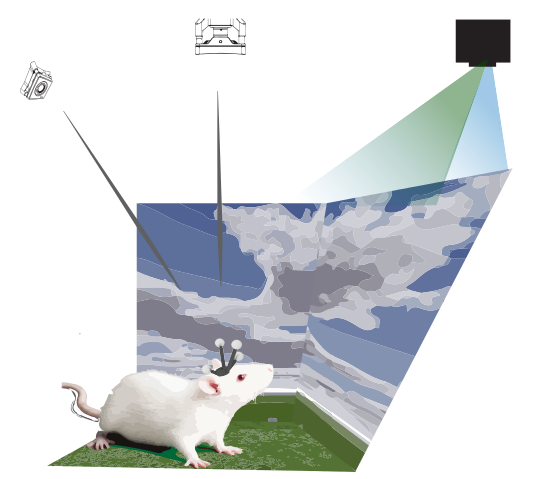
\includegraphics[width=7cm]{img/cave.png}
  \end{figure}

  
\end{frame}






\section{References}
\begin{frame}
  \frametitle{References}

  Thanks
\tiny
\nocite{*}
\bibliographystyle{apalike}
\bibliography{references}


\end{frame}




% \section{Section no. 2}
% \subsection{Lists I}
% \begin{frame}
%   \frametitle{unnumbered lists}
%   \begin{itemize}
%   \item Introduction to  \LaTeX{}
%   \item Course 2
%   \item Termpapers and presentations with \LaTeX{}
%   \item Beamer class
%   \end{itemize}
% \end{frame}

% \begin{frame}\frametitle{lists with single pauses}
%   \begin{itemize}
%   \item Introduction to  \LaTeX{}  \pause
%   \item Course 2 \pause
%   \item Termpapers and presentations with \LaTeX{}  \pause
%   \item Beamer class
%   \end{itemize}
% \end{frame}

% \begin{frame}\frametitle{lists with pause}
%   \begin{itemize}[<+->]
%   \item Introduction to  \LaTeX{}
%   \item Course 2
%   \item Termpapers and presentations with \LaTeX{}
%   \item Beamer class
%   \end{itemize}
% \end{frame}



% \subsection{Lists II}
% \begin{frame}\frametitle{numbered lists}
%   \begin{enumerate}
%   \item Introduction to  \LaTeX{}
%   \item Course 2
%   \item Termpapers and presentations with \LaTeX{}
%   \item Beamer class
%   \end{enumerate}
% \end{frame}

% \begin{frame}
%   \frametitle{numbered lists with single pauses}
%   \begin{enumerate}
%   \item Introduction to  \LaTeX{}  \pause
%   \item Course 2 \pause
%   \item Termpapers and presentations with \LaTeX{}  \pause
%   \item Beamer class
%   \end{enumerate}
% \end{frame}

% \begin{frame}
%   \frametitle{numbered lists with pause}
%   \begin{enumerate}[<+->]
%   \item Introduction to  \LaTeX{}
%   \item Course 2
%   \item Termpapers and presentations with \LaTeX{}
%   \item Beamer class
%   \end{enumerate}
% \end{frame}




% \section{Section no.3}
% \subsection{Tables}
% \begin{frame}
%   \frametitle{Tables}
%   \begin{tabular}{|c|c|c|}
%     \hline
%     \textbf{Date} & \textbf{Instructor} & \textbf{Title} \\
%     \hline
%     WS 04/05 & Sascha Frank & First steps with  \LaTeX  \\
%     \hline
%     SS 05 & Sascha Frank & \LaTeX \ Course serial \\
%     \hline
%   \end{tabular}
% \end{frame}


% \begin{frame}
%   \frametitle{Tables with pause}
%   \begin{tabular}{c c c}
%     A & B & C \\
%     \pause
%     1 & 2 & 3 \\
%     \pause
%     A & B & C \\
%   \end{tabular}
% \end{frame}


% \section{Section no. 4}
% \subsection{blocs}
% \begin{frame}
%   \frametitle{blocs}

%   \begin{block}{title of the bloc}
%     bloc text
%   \end{block}

%   \begin{exampleblock}{title of the bloc}
%     bloc text
%   \end{exampleblock}


%   \begin{alertblock}{title of the bloc}
%     bloc text
%   \end{alertblock}
% \end{frame}

\end{document}

%%% Local Variables:
%%% mode: latex
%%% TeX-master: "<none>"
%%% End:
